\chapter{Test}
\section{Time Efficiency Test}
\label{TimeEfficiencyTest}
In the beginning of this project, we made some requirements for the slideshow programming language. One of these was that the language should be faster to create slideshows in, than already existing slideshow programming languages. \\
To see whether the developed language was able to fulfil this requirement, we made a test, to see how long it would take to create slideshows in our language, and compared it to other languages and programs for creating slideshows.
\\ \\
Earlier in the report a few other slideshow solutions was mentioned; Microsoft PowerPoint, \LaTeX~Beamer and Apple Keynote. These programs will be compared to the developed language.\\
The test consists of five slides. The slides were the same on each of the tests, to make the complexity the same. The test person was one of the group members, who has experience in the developed language, and also the rest of the programs.
The result of the test is shown in table \ref{tbl:TestTable}.
\begin{table}
\centering
   \begin{tabular}{ | l | l |}
    \hline
    Program / language & Time \\ \hline
    NISSE (PC) & 09 minutes 45 seconds \\ 
    \LaTeX~Beamer (PC) & $\sim$ 45 minutes \\
    Microsoft PowerPoint (PC) & 05 minutes 55 seconds \\ 
    Apple Keynote (Ipad) & 12 minutes 40 seconds \\ 
    NISSE (Ipad) & 09 minutes 00 seconds \\ \hline
    
    \end{tabular}
    \caption{Test table}
    \label{tbl:TestTable}
\end{table}
The tests were made in the same order they occurred in the table.
\\ \\
The testing of \LaTeX~Beamer took a lot of time, because additional packages had to be installed on the test computer, and specific commands had to be found on the Internet in order to create the test slideshow.
The Microsoft PowerPoint presentation was the absolutely fastest way to create the test slideshow, but this test was mainly made to compare pointing languages with non-pointing language. This showed a huge amount of saved time compared to the rest. \\
The main result of this test is that developing the test slideshow using \LaTeX~Beamer on a PC and NISSE, showed that NISSE takes less time to create a slideshow in. NISSE beats \LaTeX~Beamer because the user has to browse the internet for certain commands and packages, while using \LaTeX~Beamer.
\\ \\
The reason that it was faster to create the test slideshow with NISSE on an Ipad than on PC might have been that the test person knew what was on the slides, after creating the same slideshow multiple times

\section{Language tests \& known errors}
To find errors or bugs in the language or compiler a series of tests have been run to verify that a given input would result in a viable output. 
Testing was done by writing many different viable constructs and combining them in different ways. Below is some of the constructs that was made, and some of the errors have been corrected due to faulty code in the compiler, others have been addressed for further development.

\begin{lstlisting}[frame=single,caption=NISSE construct,label=lst:ltest3, language=nisse]
@begin{slide}
@image{@url:http://google.com/logo.png | @i{Image text.}}
@end{slide}
\end{lstlisting}
\begin{lstlisting}[frame=single,caption=NISSE construct,label=lst:ltest31, language=nisse]
@begin{slide}
@i{@image{@url:http://google.com/logo.png | Image text.}}
@end{slide}
\end{lstlisting}
In listing \ref{lst:ltest3} the construct results in the image description being italic. That is the expected behaviour of format keywords. In listing \ref{lst:ltest31} the same construct is given but the order of format keywords is opposite so the image is defined inside an italic construct. This will result in the same as listing \ref{lst:ltest3} which is also the expected outcome.
\begin{lstlisting}[frame=single,caption=NISSE construct,label=lst:ltest1, language=nisse]
@begin{slide}
@image{@url:http://google.com/logo.png | @title{Image text as title text.}}
@end{slide}
\end{lstlisting}
\begin{lstlisting}[frame=single,caption=NISSE construct,label=lst:ltest2, language=nisse]
@begin{slide}
@title{@image{@url:http://google.com/logo.png | Image text.}}
@end{slide}
\end{lstlisting}
In listing \ref{lst:ltest1} the same image construct as in listing \ref{lst:ltest3} is given but the image description here poses as a title. This will result in the image text have the properties of a title thus not being image text. However in listing \ref{lst:ltest2} the construct order is the opposite as in listing \ref{lst:ltest31} but the outcome is not the same. Here it will not get the title property as it is the inner construct that defines which type the text will be. This is therefore also the expected outcome but it is not consistent with other format keywords behaviour in the same context.

\begin{lstlisting}[frame=single,caption=NISSE construct,label=lst:ltest4, language=nisse]
@begin{slide} 
# ordered num %\label{lst:ltest41}%
## Lorem
### ispum
#### dolor %\label{lst:ltest42}%
##### sit
#### amet %\label{lst:ltest43}%
### consectetur
## adipiscing
# elit. %\label{lst:ltest44}%
@end{slide} 
\end{lstlisting}
Listing \ref{lst:ltest4} should result in a slide with a numeration list. This is partly the result, except items are not numbered in the correct order. Expected behavior is, line \ref{lst:ltest41} would go together with line \ref{lst:ltest44} and line \ref{lst:ltest2} would go together with line \ref{lst:ltest43} however this is only true for line pair \ref{lst:ltest41} and \ref{lst:ltest44}. All other will start with 1 thus not having correct numbering. Also see image \ref{img:ltest4} for graphical representation of the outcome. This is a bug that will not be corrected at this time, but will have to be done before initial release.

\begin{figure}[H]
	\centering
		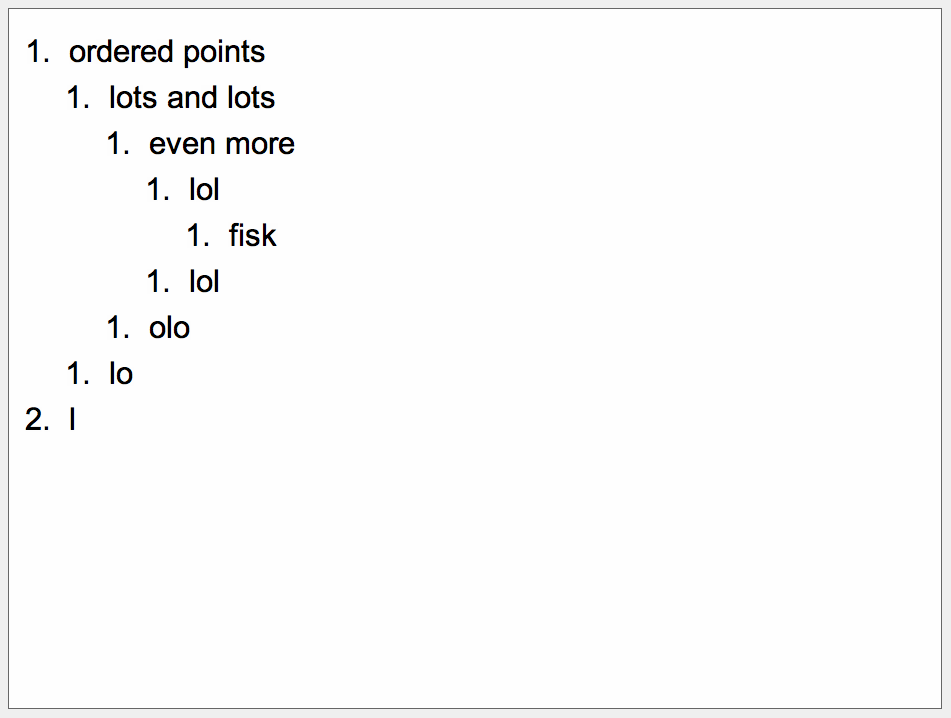
\includegraphics[width=0.8\textwidth]{images/ltest4.png}
	\caption{Incorrect numbering of numeration list}
	\label{img:ltest4}
\end{figure}

\begin{lstlisting}[frame=single,caption=NISSE construct,label=lst:ltest6, language=nisse]
@begin{slide}
��� ���
@end{slide}
\end{lstlisting}
In listing \ref{lst:ltest6} danish characters is used, but the lexer does not properly recognize these as valid tokens. This is a bug that will not be corrected at this time, but will have to be done before initial release.

\begin{lstlisting}[frame=single,caption=NISSE construct,label=lst:ltest8, language=nisse]
@begin{s} %\label{lst:ltest81}%
Slide content...
@end{s} %\label{lst:ltest82}%
\end{lstlisting}
Listing \ref{lst:ltest8} shows at line \ref{lst:ltest81} the slide name of the slide simply being one character which is the same on line \ref{lst:ltest82}. This is a valid construct according to the intended use of slide names. However in listing \ref{lst:ltest9} line \ref{lst:ltest91} and \ref{lst:ltest92} does not match each other but no error is given. This is not as intended and should be corrected before initial release. In listing \ref{lst:ltest10} line \ref{lst:ltest101} specifies a slide name that is also a valid input as a transition type, thus the slide will have that specific transition type. This is not as intended, the intention is that a pipe is given between transition type and slide name. An example of a correct input is in listing \ref{lst:ltest11}. This is also a bug which will not be corrected at this time, but should be before initial release.

\begin{lstlisting}[frame=single,caption=NISSE construct,label=lst:ltest9, language=nisse]
@begin{s}%\label{lst:ltest91}%
Slide content...
@end{f}%\label{lst:ltest92}%
\end{lstlisting}

\begin{lstlisting}[frame=single,caption=NISSE construct,label=lst:ltest10, language=nisse]
@begin{fade}%\label{lst:ltest101}%
Slide content...
@end{s}%\label{lst:ltest102}%
\end{lstlisting}

\begin{lstlisting}[frame=single,caption=NISSE construct,label=lst:ltest11, language=nisse]
@begin{fade | slideone}%\label{lst:ltest111}%
Slide content...
@end{slideone}%\label{lst:ltest112}%
\end{lstlisting}

\noindent{Other tests include how the compiler reacts to syntactically invalid slideshows and which errors is given in different error scenarios. If an error is met in the lexer or parser the compiler will stop and give an error message that explains what the error is, and how it might be corrected. If an error occurs in the semantic analysis, and in the code generator, the faulty input is simply ignored and an error is written to an error table which can be viewed by setting the appropriate debug level when compiling.}